\section{Preliminary work}
\label{sec:preliminary_work}

\subsection{Motivation}
\begin{figure}
	\centering
		
	\hfill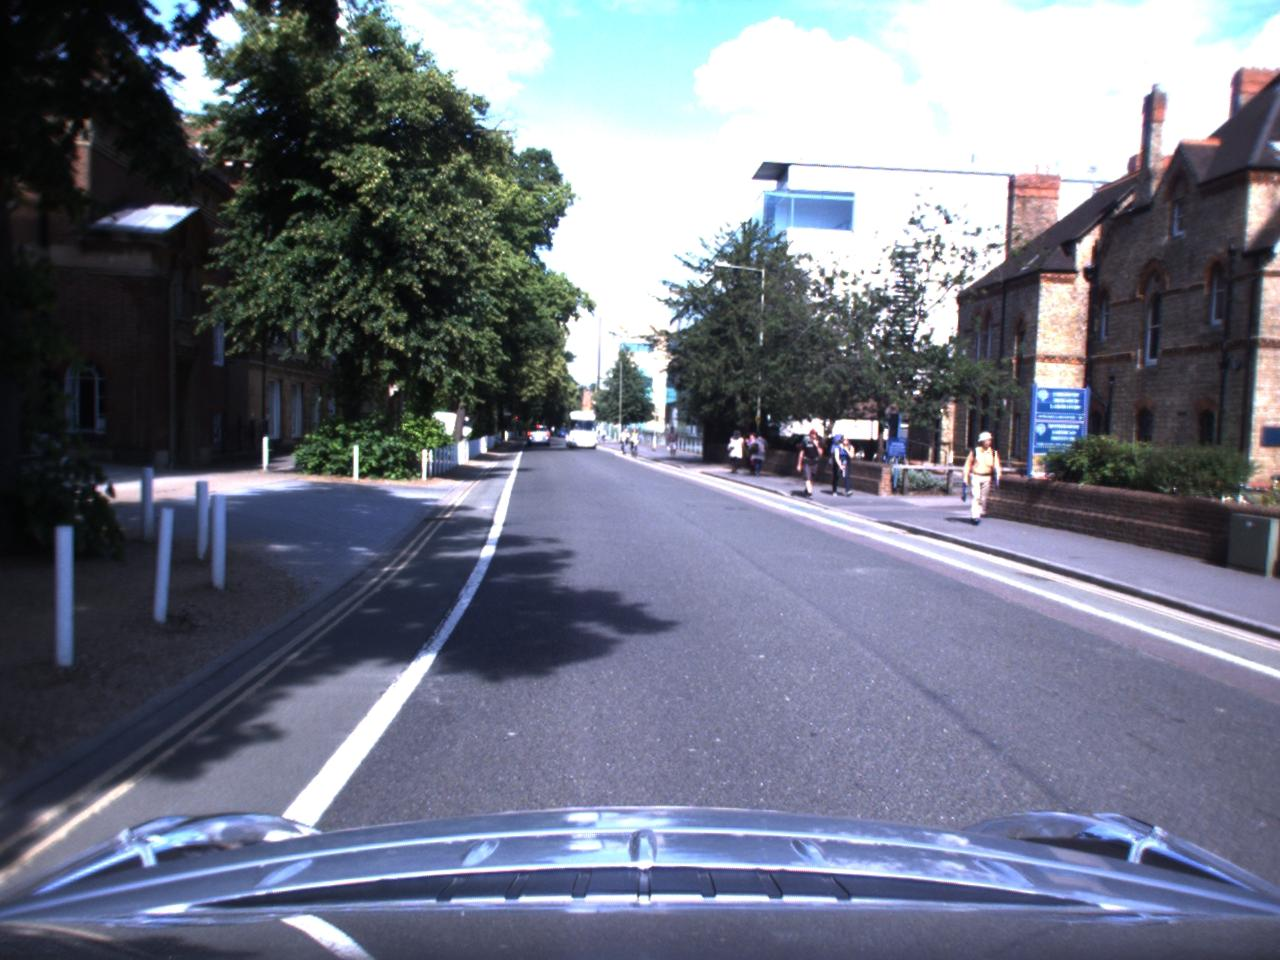
\includegraphics[width=0.25\linewidth]{preliminary/sun}\hfill
	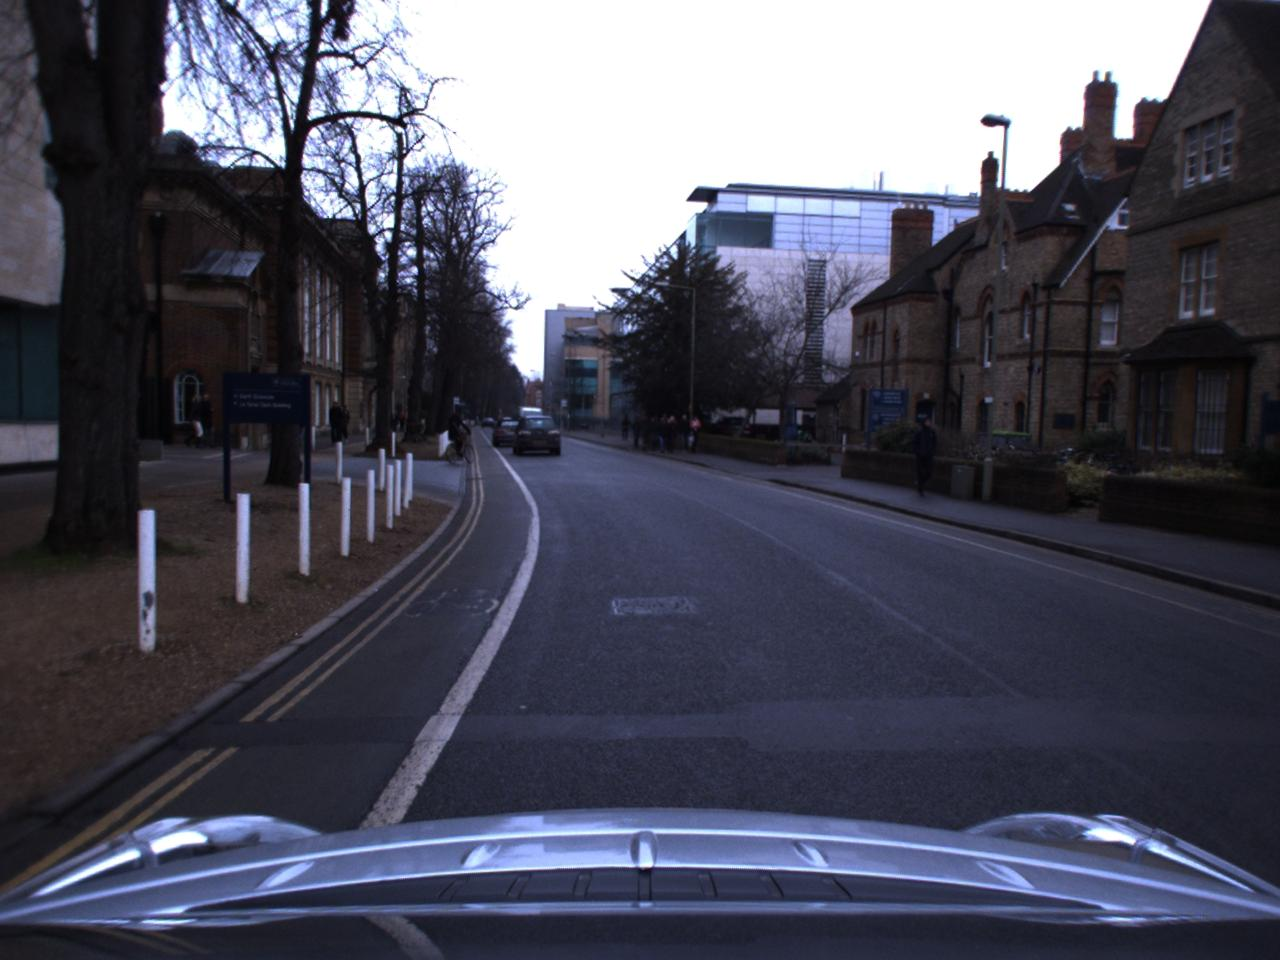
\includegraphics[width=0.25\linewidth]{preliminary/overcast}\hfill
	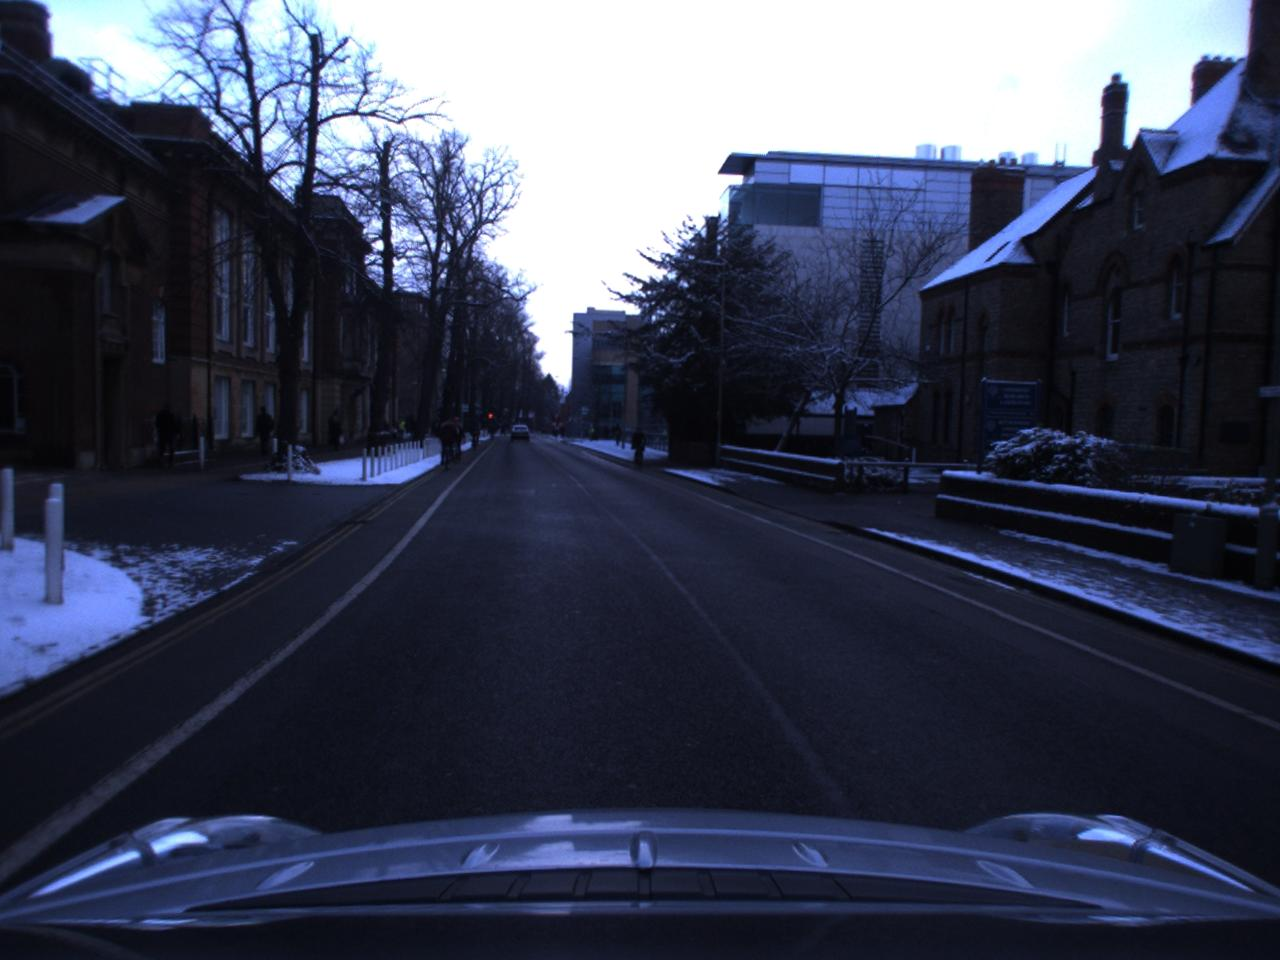
\includegraphics[width=0.25\linewidth]{preliminary/snow}\hfill
	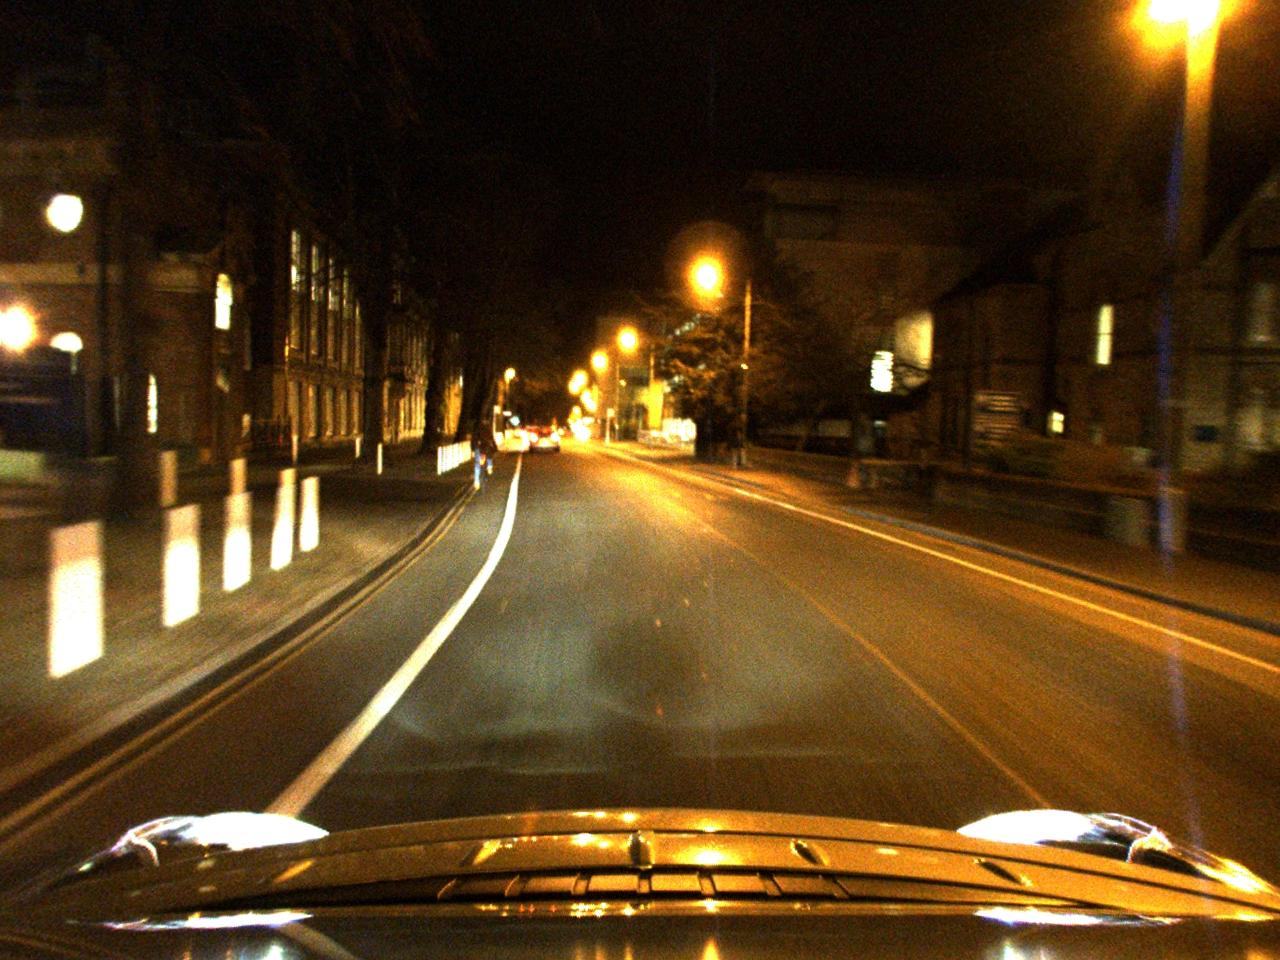
\includegraphics[width=0.25\linewidth]{preliminary/night}\hfill
	
	\hfill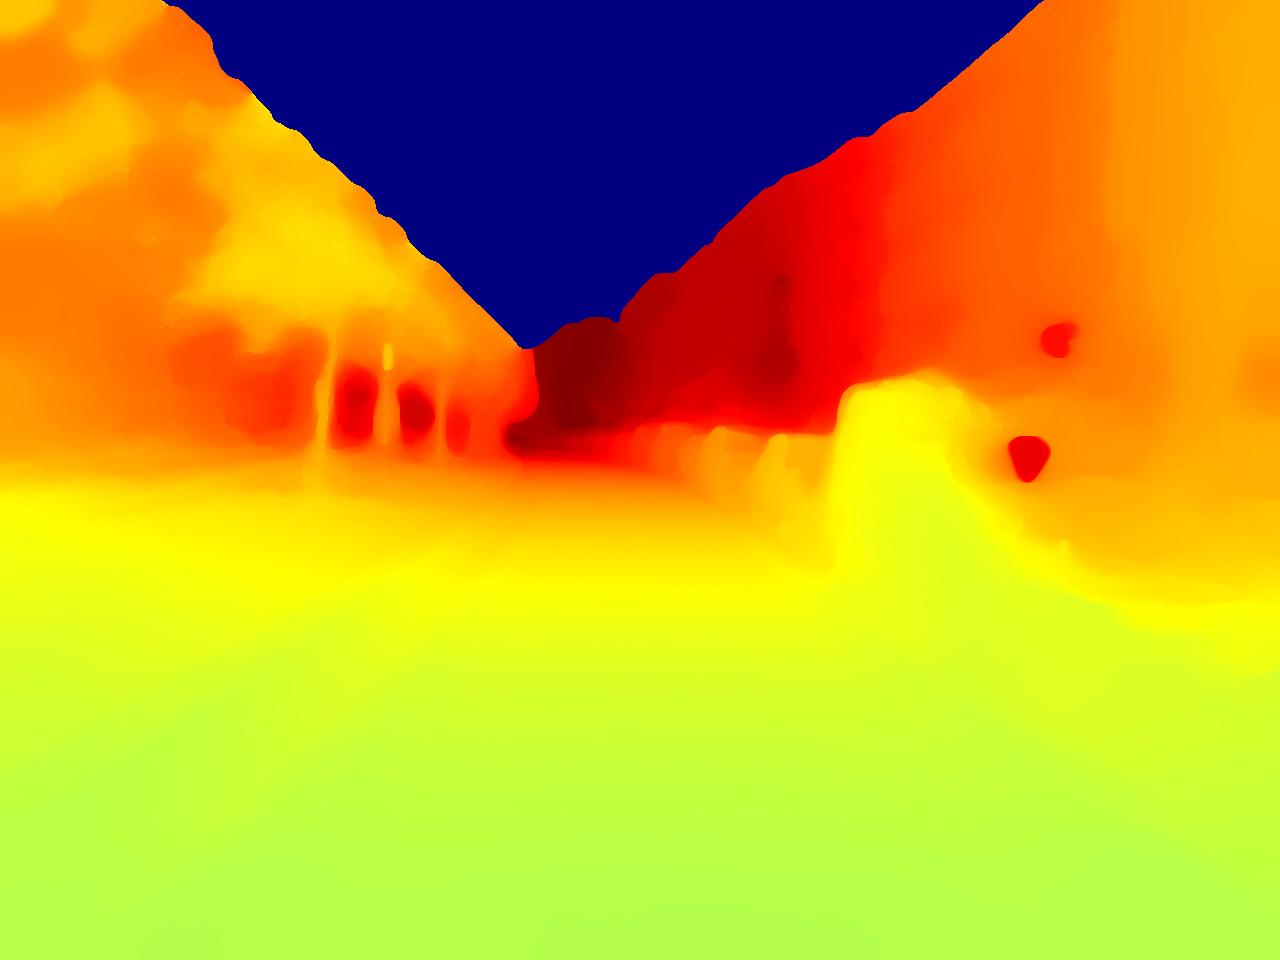
\includegraphics[width=0.25\linewidth]{preliminary/depth}\hfill
	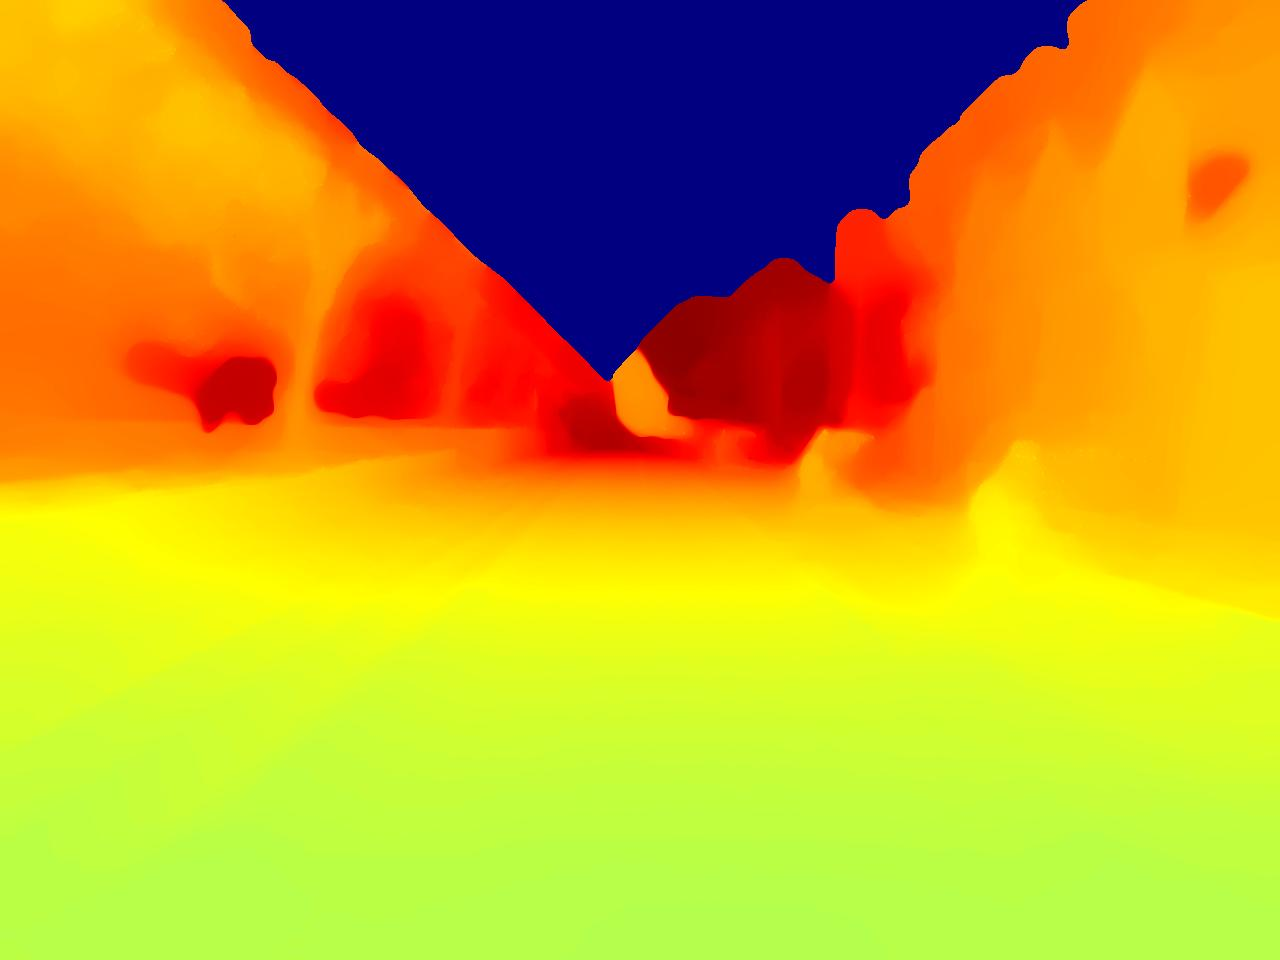
\includegraphics[width=0.25\linewidth]{preliminary/depth3}\hfill
	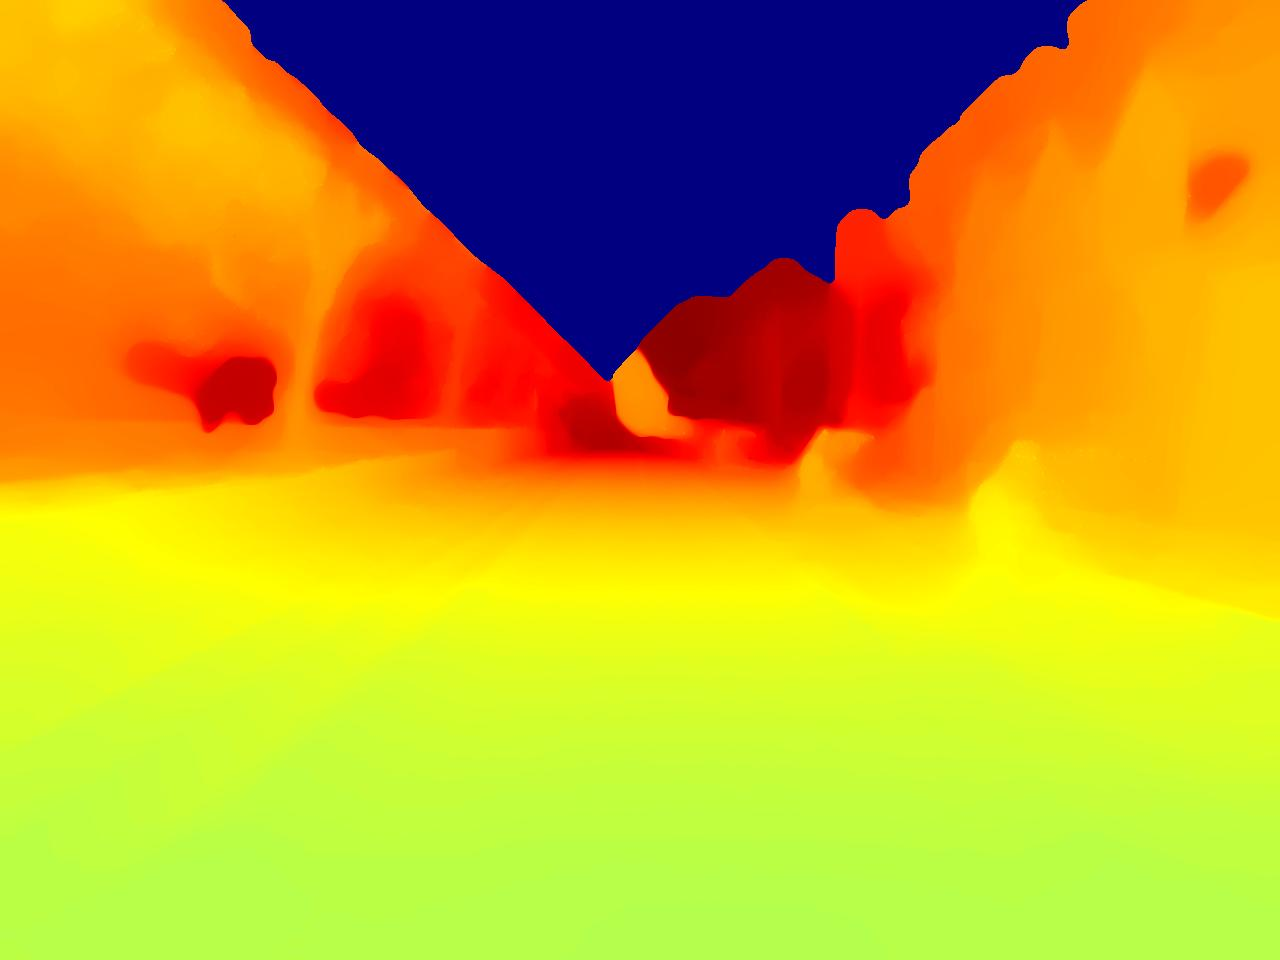
\includegraphics[width=0.25\linewidth]{preliminary/depth3}\hfill
	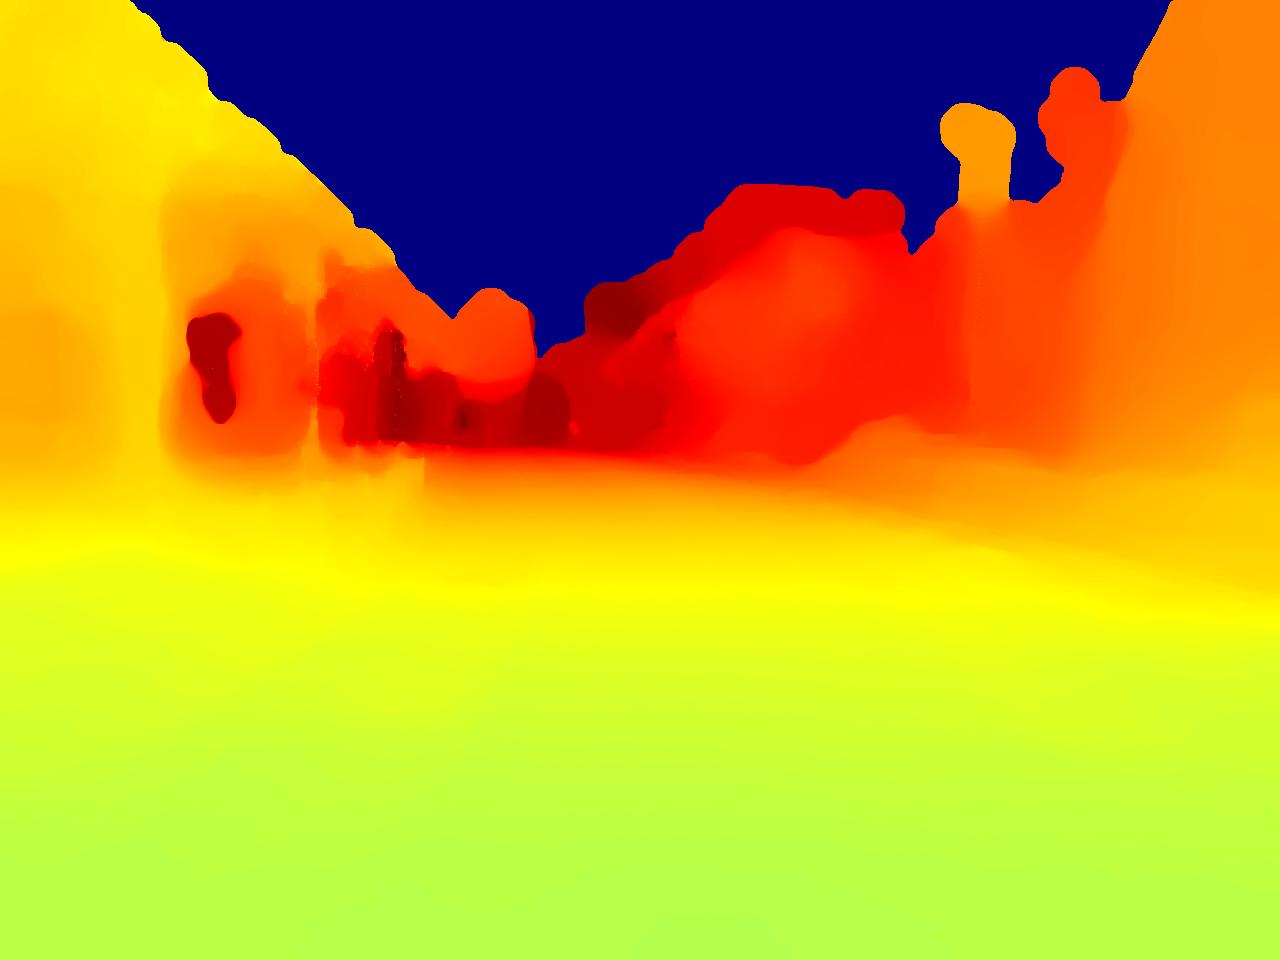
\includegraphics[width=0.25\linewidth]{preliminary/depth4}\hfill

	\caption[Images and depth maps comparison]{\label{fig:image_vs_depth} \textbf{Visual changes between radiometric and geometric domain:} due to outdoor conditions, visual aspect of images changes over time (top row), while, geometry of the scene (corresponding depth maps, bottom row) remains stable.}
	
\end{figure}
	
As illustrated in figure~\ref{fig:image_vs_depth}, outdoor conditions drastically impact visual appearance of a scene. It will be challenging for a descriptor relying only on the radiometric information to associate to the four images of figure~\ref{fig:image_vs_depth} similar embeddings. Thus, if we take a look at the underlying geometry in these images (\ie the associated depth maps, bottom of figure~\ref{fig:image_vs_depth}), this information seems more stable across changing conditions. The central idea of our method is to use recent modality transfer network~\citep{Eigen2014, Godard2017, Mahjourian2018} (from images to depth maps) to provide invariant image representation to our \ac{cnn} descriptor during training. At test time, the trained descriptor can be used on images only.

\subsection{Initial model architecture}
\begin{figure}
	\centering
	
	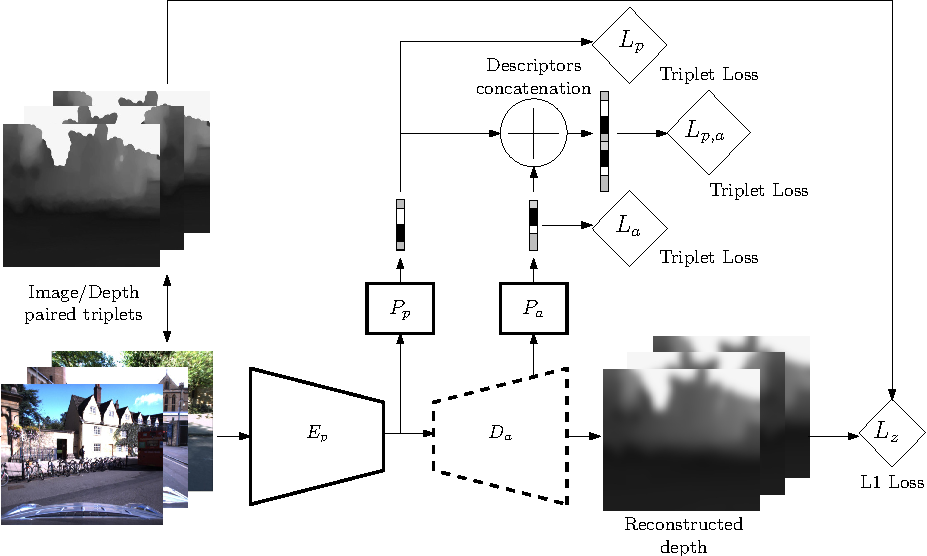
\includegraphics[width=\linewidth]{preliminary/preliminary_method}
	
	\caption[Preliminary solution]{\label{fig:preliminary_method} \textbf{Training pipeline of our preliminary solution.}}
	
\end{figure}
An overview of our method can be seen in figure~\ref{fig:preliminary_method}.

\paragraph{Principal descriptor.}
We build on recent advance in \ac{cnn} image descriptor for designing our system. We use standard convolution features extractor linked to a pooling descriptor layer (figure~\ref{fig:cnn_aggregation}). Formally, we denote $f_p$ the principal features vector of image $x$ computed by encoder $E_p$ and descriptor $P_p$:
\begin{equation}
	\label{eq:desc_details}
	f_p(x) = P_p(E_p(x)).
\end{equation}

We denote $\theta_{p}$ the weights of the image encoder and descriptor $\{E_p, P_p\}$. Notice that descriptor $P$ do not necessary contains trainable parameters (if we consider \ac{mac} pooling method for instance).

Considering the images triplet $\{x, x^+, x^-\}$, as described in previous section (see figure~\ref{fig:triplet_training}), our \ac{cnn} descriptor can be trained with the following triplet ranking loss~\citep{Arandjelovic2017}:
\begin{equation}
	\label{eq:triplet_loss}
	L_p(x, x^+, x^-) = max\left(\lambda + \norm{f_p(x) - f_p(x^+)}_2 - \norm{f_p(x) - f_p(x^-)}_2, 0 \right),
\end{equation}
where $\lambda$ is an hyper-parameter controlling the margin between positive and negative examples.

\paragraph{Side geometry learning.}
In order to recover the geometric information from the radiometric signal, we use a fully convolutional decoder $D_a$~\citep{Eigen2014}. $\theta_{a}$ are the trainable weights of our decoder. Lets $\{x, z\}$ be a pair of image and corresponding depth map, we can train our decoder to compute the depth map from input image with the following loss function:
\begin{equation}
	\label{eq:l1_loss}
    L_z(x,z) = \norm{z - \hat{z}(x)}_{1},
\end{equation}
where $\hat{z}(x) = D_a(E_p(x))$, is the output of the decoder. $L_z$ is a simple pixel loss penalizing absolute error between the output depth map $\hat{z}(x)$ and the target $z$.

\paragraph{Auxiliary descriptor.}
In order to take advantages of the learned depth representation in our final descriptor, we use intermediate deep features computed by $D_a$ to create another descriptor $f_a$:
\begin{equation}
	\label{eq:desc_aux}
	f_a(x) = P_a(\bar{D}_a(E_p(x))),
\end{equation}
where $P_a$ is an auxiliary descriptor and $\bar{D}_a$ designs an intermediate output extracted from decoder $D_a$. We do not use the reconstructed depth map $\hat{z}(x)$ (\ie raw output of $D_a$) to produce vector $f_a(x)$ because it will be to sensitive to small viewpoint variations. Instead, we use an intermediate output from $\bar{D}_a$, that should be more meaningful compared to  $\hat{z}(x)$ and less sensitive to viewpoint changes. Indeed, because the decoder upsample the features maps, output of $\bar{D}_a$ has a smaller spatial resolution and is deeper in comparison to $\hat{z}(x)$. We apply a triplet ranking loss $L_a$ (see equation~\ref{eq:triplet_loss}) to train weights $\theta_{a}$ of decoder $D_a$ and descriptor $P_a$. 

\paragraph{Overall training.}
Finally, we combine the principal and auxiliary features, $f_p(x)$ and $f_a(x)$ in a common vector:
\begin{equation}
	\label{eq:concat_desc}
	f_{p,a}(x) = \left[ f_p(x), f_a(x)  \right],
\end{equation}
where $[ \cdot ]$ is the concatenation operation. Overall optimization is obtained through the last triplet ranking loss $L_{p,a}$ and the final cost function is defined by:
\begin{multline}
	\label{eq:overall_loss}
	L(x, x^+, x^-,z, z^+, z^-) = L_p(x, x^+, x^-) + L_a(x, x^+, x^-) + L_{p,a}(x, x^+, x^-)\\
	 + \frac{1}{3}\left[ L_z(x, z) + L_z(x^+, z^+) + L_z(x^-, z^-) \right].
\end{multline}

Our initial method requires triplets of RGB-D data to be trained.

\subsection{Hallucination network}
\begin{figure}
	\centering
	
	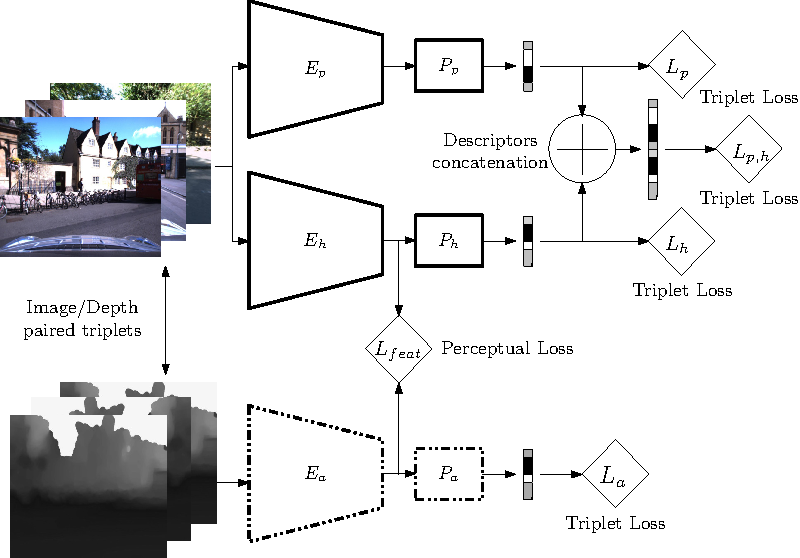
\includegraphics[width=\linewidth]{preliminary/hall_method_training}
	
	\caption[Hallucination network for image descriptors learning]{\label{fig:hall_method} \textbf{Hallucination network for image descriptors learning:} we train an hallucination network, inspired from~\cite{Hoffman2016}, for the task of global image description. Unlike the proposed method (see figure~\ref{fig:our_method}), hallucination network reproduces feature maps that would have been obtained by a network trained with depth map rather than the deep map itself.}
	
\end{figure}

We compare our method of side information learning with a state-of-the-art approach system, named hallucination network~\citep{Hoffman2016}. The hallucination network was originally designed for object detection and classification in images and have never tested for image description task. We adapt the work of~\citet{Hoffman2016} to create an image descriptor system that benefits from depth map side modality during training. Our adaptation of the hallucination network for image description is presented in figure~\ref{fig:hall_method}.

\paragraph{Principal descriptor.}
Similar to our proposal, the system is composed of a principal image descriptor: encoder $E_p$ + descriptor $P_p$, trained jointly through triplet ranking loss of equation~\ref{eq:triplet_loss}.

\paragraph{Auxiliary descriptor.}
Hallucination architecture needs an auxiliary network for training purpose, that will be discarded at test time. This auxiliary branch focus on extracting significant information from the side modality (the depth map in our case). We design the auxiliary network similar to our principal branch: the depth map descriptor is composed of an encoder $E_a$ linked to a descriptor $P_a$. The depth map descriptor is trained with a triplet ranking loss $L_a$, where the embeddings are directly computed from the truth depth maps:
\begin{equation}
	f_a(z) = P_a(E_a(z)).
\end{equation}

\paragraph{Hallucination descriptor.} The key component of \citet{Hoffman2016} proposal is the hallucination network. The task of the hallucination branch is, with images as input, to reproduce feature maps that would have been obtained by a network trained with depth map rather than the depth map itself. The hallucination network share the same architecture as the principal and the auxiliary branches. The hallucination descriptor is composed of an encoder $E_h$ and a descriptor $P_h$ with trainable weights $\theta_h$. It is trained with triplet ranking loss $L_h$ under the constraint of a perceptual loss~\citep{Johnson2016}:
\begin{equation}
	\label{eq:perceptual_loss}
	L_{feat}(x, z) = \norm{E_h(x) - E_a(z)}_2.
\end{equation}
This constraint can be interpreted as knowledge distillation~\citep{hinton2015distilling}. Final image descriptor is obtained by concatenating $f_p(x)$ and $f_h(x)$.

\paragraph{Overall training.} Training routine presented in~\citep{Hoffman2016} is two-step: we first train weights $\theta_a$ of the auxiliary descriptor with loss $L_a(z, z^+, z^-)$ and, secondly, we initialize hallucination weights $\theta_h$ with pre-trained weights $\theta_a$ and minimize the following cost function:
\begin{multline}
	\label{eq:overall_hall_loss}
	L(x, x^+, x^-,z, z^+, z^-) = \alpha\left[ L_p(x, x^+, x^-) + L_h(x, x^+, x^-) + L_{p,h}(x, x^+, x^-) \right]\\
	+ \gamma\left[ L_{feat}(x, z) + L_{feat}(x^+, z^+) + L_{feat}(x^-, z^-) \right],
\end{multline}
where $\alpha$ and $\gamma$ are weighting constants. During final optimization, weights $\theta_a$ are frozen. 

Like our proposal, this method requires triplets of RGB-D data to be trained and, at test time, the principal and hallucination descriptors are used on images only.

\subsection{Discussion}

Exploratory testing of our method has lead to unsuccessful results. During the training step, our network fails to produce at the same time a meaningful image representation for localization (losses $L_p$, $L_a$ and $L_{p,a}$) and to reconstruct the scene geometry (loss $L_z$). After analyzing our architecture, we came up with the following conclusions: the two target objectives are disrupting each other. This problem is due to the design of our method: error back-propagation from triplet ranking losses are affecting both weights of encoder $E_p$ and decoder $D_a$, as same as error computed by $L_z$ in equation~\ref{eq:l1_loss}. 

We do not encounter the same problem with our implementation of hallucination network. The only loss functions that can interfere during the optimization are triplet ranking loss $L_h$ and perceptual loss $L_{feat}$. Both losses lead to modification of hallucination encoder $E_h$ weights. But targeted task of the two loss function are the same: $L_h$ directly optimize the hallucination embedding for image retrieval and $L_{feat}$ force the features maps of encoder $E_h$ to be close to the features maps of encoder $E_a$, an encoder that have been trained for image retrieval task as well.

In the next section, we propose an improved version of our initial method that solves the aforementioned issue.